\section{\seamlessexpressive}
\label{sec:expressivity}



Prosody contains rich paralinguistics functions in human communication, such as portraying a speaker's emotional state, attitude, and intent. How a speaker says an utterance can dramatically alter its meaning (holding semantic content constant). For instance, humans leverage variations in pitch (high or low), loudness (strong or soft), and duration (fast or slow) to express themselves in different situations.













In this section, we describe how we built \seamlessexpressive, a model that captures certain underexplored aspects of prosody, such as speech rate and pauses, while preserving the style of one's voice and high content translation quality.
More specifically, we developed \seamlessexpressive with the following techniques: 
\begin{enumerate*}[label={\arabic*})]
    \item we leveraged \mfourttwo as a foundational model to achieve high accuracy in translation quality from a semantics standpoint,
    \item we proposed \textbf{\prosodyunitytwo}, integrating an expressivity encoder in \mfourttwo to guide unit generation with proper rhythm, speaking rate and pauses, and
    \item we replaced the unit HiFi-GAN vocoder in \mfourttwo with \textbf{\ptv}, an expressive unit-to-speech generator conditioned on the source speech for waveform generation to transfer tones, emotional expression, and vocal style.
\end{enumerate*}


\seamlessexpressive, which preserves not only sentence-level rhythm and tone but also token-level prosody such as pauses, required prosody-aligned parallel speech data for \prosodyunitytwo training. As a result, we describe our effort to collect hours of prosody-aligned parallel speech data in six high-resource languages—English, French, German, Italian, Mandarin, and Spanish.


\subsection{Expressive Speech-to-Speech Translation Data}
\label{sec:expressive_data}
In this section, we introduce our efforts on collecting prosody-aligned parallel speech through data commissioning, automatic alignment, and synthesizing. Commissioned data, including mExpresso and mDRAL, are well-aligned in emotions but limited in data size and diversity. We explore large-scale expressive aligned data—finding expressivity preserving cross-lingual alignments between speech segments from corpora. Finally, synthetic data is part of our data augmentation strategy with \sonar, controllable TTS (cTTS), and \unitvb, which contributed a large amount of aligned expressive speech.




\subsubsection{mExpresso}
\label{subsec:mexpresso}

The Expresso corpus \citep{nguyen2023expresso} is an English expressive speech dataset that includes both expressively rendered read speech (comprising eight styles) and improvised dialogues. We created mExpresso, a multilingual version of Expresso, by expanding six styles of read speech (i.e., default, happy, sad, confused, enunciated, and whisper) to five other languages—French, German, Italian, Mandarin and Spanish. %

To expand the Expresso dataset, bilingual translators first translated the English transcriptions into other languages, including the emphasis markers in the transcription. Second, a different set of gender-matched bilingual speakers (native in the target languages) read the translation in the style suggested by the markers. The speakers had access to the original English recordings to learn how a sentence was uttered initially. To control the quality of the recording, a different set of bilingual reviewers reviewed each recording to check the expressiveness preservation and recording quality, and the speakers re-recorded utterances until all recordings passed the quality check.




\subsubsection{mDRAL}
\label{subsec:mDRAL}



Dialogues Re-enacted Across Languages (DRAL) Corpus, proposed in~\citet{ward2023dral}, is a bilingual speech corpus of parallel utterances in Spanish and English created by recording spontaneous conversations and fragments re-enacted by bilingual speakers in a different language.
More specifically, during a recording, two speakers were instructed to carry out unscripted conversations. The moderator then selects ``interesting'' fragments, which are utterances that elicited more active engagement between the speakers and guided the speakers to re-enact.

We followed the data collection protocols described in~\citet{ward2023dral}, expanded the collection to native speakers of French, German, Italian, Mandarin, or Spanish who are proficient in English, and created the multilingual DRAL corpus dubbed mDRAL (see \Cref{sec:expressive_data_collection} for an overview of the collection protocol).
Unlike the original DRAL collection, we performed the collection remotely with the moderator and the two speakers meeting over Zoom. One challenge in scaling up the data collection effort is the throughput—the number of meaningful speech segments we can acquire from each conversation. We provided the speakers with 32 emotion categories found in EmpatheticDialogues~\citep{rashkin2019towards} as topic prompts to increase data collection efficiency. Compared to mExpresso, mDRAL has less exaggerated and performed emotions, while the prosody is more natural.



\subsubsection{Automatically extracting expressive audio alignments}
\label{subsec:exp_audio_alignment}


Speech-to-speech pairs that are automatically aligned based on semantics (like \seamlessalign), %
do not always contain the same expressive characteristics. 
While a simple filtering approach %
based on heuristics could be devised, the volume of the resulting dataset would likely be drastically reduced as no explicit prosody-preservation goal was enforced to begin with (i.e., data would be expressively aligned by chance). Instead, we chose to modify the algorithm of \seamlessalign to not only seek alignments based on semantic preservation but also to incorporate prosodic similarity.

The core algorithm behind \seamlessalign relies on the computation of a semantic-based margin score (see \Cref{sec:offline:data}). We supplement that semantic score with the result of an auxiliary model capable of determining prosodic similarity. 
Based on these two components, we introduce a new weighted scoring function defined as:

\begin{equation}
    \label{eqn:blended_score}
    \text{blended-score}(x, y) = \alpha \cdot \text{margin} + (1 - \alpha) \cdot \text{prosody-score}.
\end{equation}

\noindent Given the above formulation, an overview of the expressive audio alignment is shown in \Cref{fig:expressive_alignment_process}. We began with the same process as \seamlessalign by semantically retrieving the k-nearest neighbors in a multilingual embedding space. Then, instead of choosing a neighbor with the best margin (i.e., semantic score), we applied a prosodic-based auxiliary model to each neighbor and chose a candidate with the highest blended score as defined in \Cref{eqn:blended_score}.

\begin{figure}[!tbh]
    \centering
    \hspace{-50pt}\begin{minipage}[t]{\textwidth}
        \includegraphics[width=1.1\linewidth]{figures/data/expressive_alignment_process.png}
    \end{minipage}
    \caption{\textbf{Expressive audio alignment process.} Similar to \seamlessalign, audio was first language-identified and over-segmented, and then the resulting segments were embedded into a multilingual embedding space. k-nearest neighbor candidates were then retrieved based on the semantic-based margin and subsequently re-ranked with the blended score, resulting in expressively- and semantically-aligned pairs.}
    \label{fig:expressive_alignment_process}
\end{figure}

In order to tune the $\alpha$ hyperparameter in the blended score, which controls the trade-off between semantic accuracy and prosody preservation, we introduce a new proxy metric for expressive audio alignment: \xsimexp. This new benchmark builds upon \xsim, introduced in \citet{nllb2022}. Unlike \xsim, where the goal is to reconstruct a dataset through semantic-only audio alignment and measure the percentage of incorrect alignments, \xsimexp instead applies the same re-ranking as described in \Cref{eqn:blended_score} and aims to reconstruct a dataset both semantically and expressively. We applied \xsimexp to the mExpresso dataset (see \Cref{subsec:mexpresso}). Our choice was driven by a need for variety. For one, mExpresso contains sentences repeated multiple times with varying prosody. This makes it a challenging dataset for expressive audio alignments, as multiple candidates with identical semantics will be retrieved during the $k$-nearest neighbor search. On the contrary, a prosody-aligned dataset with no repetition would offer no such challenge, as alignments could be recovered based on semantic features only.



Results from \xsimexp on the mExpresso benchmark dataset are shown in \Cref{tbl:expressivity:p_xsim_results}. We tuned $\alpha$ using a grid search. To help our explorations, we also collapsed the mExpresso classes into three coarse emotion labels similar to \citet{parry2019analysis}: \emph{positive} (happy, laughing), \emph{negative} (sad, confused), and \emph{neutral} (default, whisper, enunciated). As a baseline, we used the margin score only and then tried several auxiliary models for the prosody score, namely \comparator\footnote{For expressive audio alignment, we used an earlier version of the \comparator model. It has the same architecture as the model we used for evaluation and it uses embeddings from a different layer of the XSL-R speech encoder.} (\Cref{sec:comparator}), 
and different embedding layers extracted from w2v-BERT. Adding a prosody-aware component to the audio alignment scoring function clearly boosted performance, and \comparator provided significantly higher quality alignments than representations from w2v-BERT. 

\begin{table}[!hbtp]
\small
    \centering
    \begin{tabular}{@{}lccc}
    \toprule
                           & \multirow{2}{*}{\bf \makecell{ Opt. param. \\ $\alpha$ }} & \multicolumn{2}{c}{\bf $\downarrow$ \xsimexp} \\\cmidrule{3-4}
                           &           & all emotions                  & pos/neg/neu                 \\
    \midrule
    semantic-only baseline & -                                 & 84.86                         & 60.57                       \\
    w2v-BERT - layer 23     & 0.2                              & 84.79                         & 60.27                       \\
    w2v-BERT - layer 20     & 0.1                             & 54.40                         & 36.04                       \\
    \comparator      & 0.1                              & \textbf{47.06}                & \textbf{28.90}                       \\
    \bottomrule
    \end{tabular}
    \caption{\textbf{Performance of \xsimexp.} Error rate when recreating gold alignments of various prosody-aware auxiliary scorers on the Spanish$\shortrightarrow$English mExpresso test set.} 
    \label{tbl:expressivity:p_xsim_results}
\end{table}

\noindent 
Once the $\alpha$ parameter was optimized using \xsimexp, we ran expressive \sst audio alignment at scale on a curated selection of publicly available data in our target languages. The resulting alignments were used to supplement the final training data for \seamlessexpressive.


\paragraph{\seamlessalignexpressive} Separate to the data used to train \seamlessexpressive, we apply this expressive alignment method at scale on a different publicly available corpus. The total number of hours collected can be found in \Cref{tab:expressivity-num-hours-per-dataset}. We release the metadata of this data set to the community as \seamlessalignexpressive to foster future research in expressive speech-to-speech translation as well as to validate the effectiveness of our expressive alignment method.

Upon manual inspection, we identified several emerging properties when several semantically viable candidates were available: 
\begin{itemize}
    \item expressive audio alignment seems to remove candidates with mismatched background music,
    \item emotion/intonation imbalance is highly reduced, and
    \item segments with singing are also much less common in final alignments.
\end{itemize}
While further analysis of those properties was out of the scope of this study, we hypothesized that expressive audio alignment could also have a net-positive effect on non-expressive speech translation, as it produced much cleaner alignments overall.



\subsubsection{Extracting parallel segments from videos}
\label{sec:dubbed_data}
We also processed videos in multiple languages to extract bilingual expressive segments.
This process is different from the standard audio alignment approach described in \Cref{sec:offline:data} because the audio data is almost parallel in this case.
The task is then to segment and monotonically align the multilingual audio content.

The process was performed as follows: the audio was extracted from the video, segmented, and transcribed with Whisper \citep{whisper}.
One issue we faced is that the segmentation provided by Whisper is often inconsistent across languages.
Therefore, the segments cannot be matched directly, leading to a low recall.
To solve this issue, we took advantage of the word boundaries provided by Whisper and adopted a split-merge approach, which consists of first splitting the current segments based on the pauses (available by analyzing the transcriptions) and then concatenating them back together to form new overlapping segments.
Segments longer than 25 seconds and segments having pauses longer than 1.5 seconds were excluded.
Then, the speech segments and their transcriptions were each encoded separately with our encoders
to produce two embeddings per segment.
The next step was to align the segments. If they were disjointed, we could use a simple monotonic alignment algorithm.
Yet, if not the case, finding an optimal solution would be intractable due to the large number of alignments to consider.
Therefore, we used a greedy algorithm that matched bilingual segments having the highest overall score, removed all overlapping segments from the pool, and repeated the process until the candidate pool was empty.
Each segment pair candidate was associated with a score corresponding to an average of the cosine similarities of both the text and speech embeddings. 
This score was modified according to an estimation of the lag (i.e., the time gap between the centers of both segments).
Finally, all matching candidates were filtered based on predefined rules (defined by manually inspecting the data), such as similarity threshold, duration mismatch, and time gap. %
\Cref{tbl:expressivity:video_data} shows the statistics of the resulting aligned data.

\begin{table}[!hbtp]
\small
    \centering
    \begin{tabular}{@{}lrrrrr}
        \toprule
        {\bf Language} & \MC{2}{c}{\bf Total hours} & \multirow{2}{*}{\bf \# segments} & \MC{2}{c}{ \makecell[c]{{\bf Avg. segment} \\ {\bf duration (s) } }} \\ \cmidrule{2-3}\cmidrule{5-6}
                       & { English} & { Lang.}  &                   & { English} & { Lang.} \\
        \midrule
        French &  300.7 & 299.1 & 499.0k & 2.17 & 2.16 \\
        German &  118.8 & 121.8 & 224.2k & 1.91 & 1.96 \\
        Italian &   69.3 &  68.1 & 122.4k & 2.04 & 2.00 \\
        Mandarin &  254.9 & 286.1 & 268.5k & 3.42 & 3.84 \\
        Spanish &  242.6 & 237.9 & 363.4k & 2.40 & 2.36 \\
        \bottomrule
    \end{tabular}
    \caption{\textbf{Statistics of aligned audio data}. The total duration and average segment length per language are reported for data obtained from aligning multilingual videos.} 
    \label{tbl:expressivity:video_data}
\end{table}


\label{subsection:sonar-expressive}
\subsubsection{SONAR expressive}


SONAR is a multilingual and multimodal fixed-sized sentence embedding space introduced by \citet{Duquenne:2023:sonar_arxiv}. The modalities cover both text and speech representations. However, this space is primarily grounded in text as it was tuned on speech-to-text
and text-to-text datasets. Given this grounding in text, the space is centered on semantics, so the existing \sonar space is not explicitly tuned to encode anything other than semantics from the input text or speech. \sonarexp \citep{Duquenne:2023:sonarexp_arxiv} extends the capabilities of this space to also include representations for prosodic characteristics.  

An overview of the architecture of \sonarexp is shown in \Cref{fig:sonar-expressive-architecture}. It comprises two encoders: a frozen \sonar text/speech encoder to capture semantics (\sonar embedding) and a trainable speech encoder that captures speech properties other than semantics (\speechprop embedding). Then, given a combination of both the \speechprop vector (i.e., prosody, etc.) and the semantic vector, the objective is to reconstruct the input speech, represented using EnCodec units \citep{Defossez2022HighFN}.

\begin{figure}[htp!]
    \centering
    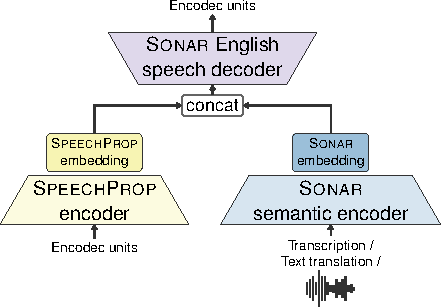
\includegraphics[width=.5\linewidth]{figures/expressivity/architecture_sonar_expressive.pdf}
    \caption{\textbf{Model architecture for \sonar Expressive.}}
    \label{fig:sonar-expressive-architecture}
\end{figure}

\noindent Given that \sonarexp has the ability to expressively decode input speech, we leveraged this as another data source for model training. We began with unaligned speech segments, %
applied the same pre-processing as used for \sonarexp model pre-training \citep{Duquenne:2023:sonar_arxiv}, and randomly sampled segments from each non-English language (French, German, Italian, Mandarin, and Spanish). As we observed that semantic preservation for the \sonar semantic encoder was higher given an English text-based input \citep{Duquenne:2023:sonar_arxiv}, segments from each non-English language were translated into English text using the \sonar encoders/decoders. Each non-English speech segment and English text translation were then expressively decoded into English. An overview of the decoded data is shown in \Cref{tab:sonar-expressive-statistics}.

\begin{table}[htp!]
    \centering
    \small
    \begin{tabular}{@{}lrrrr}
        \toprule
        {\bf Language} & \multicolumn{2}{c}{\bf Total hours} & \multicolumn{2}{c}{ \makecell[c]{{\bf Avg. segment} \\ {\bf duration (s)}} }\\ \cmidrule(r){2-3}\cmidrule(l){4-5}
                       & { English} & { Lang.}           & { English} & { Lang.}\\
        \midrule
        French &  1,651 & 1,784 & 2.97 & 3.22 \\
        German &  1,622 & 1,865 & 2.92 & 3.36\\
        Italian &  1,562 & 1,891 & 2.82 & 3.41 \\
        Mandarin &   1,672 & 1,694 & 3.02 & 3.06 \\
        Spanish &  1,567 & 1,841 & 2.83 & 3.33 \\
        \bottomrule
    \end{tabular}
    \caption{\textbf{Statistics of data decoded with \sonar Expressive.}}
    \label{tab:sonar-expressive-statistics}
\end{table}

\subsubsection{Controllable TTS (cTTS) data augmentation}
\label{ctts_aug}


One limitation of automatically aligned expressive data is that the prosody of the audio data may not be perfectly aligned between source and target speech (e.g., speech rate and pause location).
A controllable TTS (cTTS) system is able to control the speech rate and pause location of the synthesized speech from the text prompt. Therefore, we leveraged controllable TTS to synthesize more prosody-aligned speech-to-speech data.

We first sample English monolingual text to augment from. Then, we inserted one paired quote into each English text and ran NLLB~\citep{nllb2022} Dense-3.3B model for translating into all five languages (French, German, Italian, Mandarin, and Spanish).
Followed by further filtering on the translation output to ensure only one paired quote exists, we randomly replaced the paired quote in the source and target text with one of the three augmentation instructions: 1) no augmentation, 2) equal chance to insert the pause at the first or second quote, with a randomly chosen pause duration between 0.3 and 1.5 seconds and the quote converted to a special pause token. 
We used an internal controllable TTS system for all languages except Mandarin Chinese. 
For Mandarin Chinese, we trained a VITS~\citep{kim2021conditional} model on 15-hour speech data. %
We used these systems to synthesize speech with a random utterance-level speech-rate manipulation between 70\% and 130\%.



\subsubsection{Comparing across data sources}

\begin{table}[htp!]
    \centering
    \footnotesize
    \begin{tabular}{lcccccc}
        \toprule
         & \multicolumn{2}{c}{\textbf{Commissioned}} & \multicolumn{2}{c}{\textbf{Automatically Aligned}} & \multicolumn{2}{c}{\textbf{Synthetic}} \\
         \cmidrule(l){2-3}\cmidrule(lr){4-5}\cmidrule(r){6-7}
         & {mExpresso} & {mDRAL} & \begin{tabular}{@{}c@{}} { Expressive} \\ {Alignments} \end{tabular} &
         \begin{tabular}{@{}c@{}} {Video} \\ {Alignments} \end{tabular} & \begin{tabular}{@{}c@{}} {\sonar} \\ {Expressive} \end{tabular} &     {cTTS}\\
        \midrule
        Style & acted & spontaneous & spontaneous & acted & \begin{tabular}{@{}c@{}} spontaneous and \\ synthetic pairs \end{tabular} & synthetic \\
        \makecell[l]{Speaker\\diversity} & low & low & high & medium & high & low \\
        Expressiveness & high & medium & medium & high & medium & low \\
        \midrule
        \multicolumn{7}{l}{\makecell [l]{ Expressivity  alignment} }\\
        \midrule
        \makecell [l]{  Sentence-level \\ style} & \greencheck & \greencheck &  \greencheck & \greencheck & \greencheck& \redxmark\\
        speech rate  & \greencheck & \greencheck & \redxmark & \redxmark & \redxmark & \greencheck \\
        pause & \redxmark & \greencheck & \redxmark & \redxmark & \redxmark & \greencheck\\
        same voice & \redxmark & \greencheck & \redxmark & \redxmark & \greencheck & \greencheck\\
        \bottomrule
    \end{tabular}
    \caption{\textbf{Datasets characteristics.} We compare commissioned, automatically aligned, and synthetic data on style, speaker diversity, expressiveness, and sentence-level prosody alignment.
    }
    \label{tab:expressivity-data-analysis}
\end{table}


\Cref{tab:expressivity-data-analysis} describes the characteristics of each dataset in four aspects: style, speaker diversity, expressiveness, and expressivity alignment.
Spontaneous style indicates that the speech is more natural, while acted speech implies that the speech can be more expressive yet less natural.
The commissioned datasets have the lowest speaker diversity because the data collection was expensive and time-consuming.
While expressive alignment can provide a large amount of parallel data, such speech pairs are mostly aligned in sentence-level styles due to the choice of prosody score. Further filtering can be done to refine the datasets to be better aligned in speech rate and pauses.
In theory, video alignment should generate speech pairs with the best expressivity alignment. However, we find that due to the constraint of time alignment in videos and the characteristics of different languages, speech for some languages may be much faster than others.
Controllable TTS data provides speech pairs that have the best alignment in speech rate and pauses, but the speech is monotonic and lacks sentence-level expressiveness such as emotions.


\subsubsection{Training data pre-processing}
\label{subsection:expressive-data-processing}

Once data was collected, we then performed the following augmentations in order to form (source-target) speaker-aligned, clean speech data with transcriptions: (1) denoising, (2) silence removal, (3) transcription, and (4) vocal style conversion. Since datasets come from various sources (with varying audio qualities), not all preprocessing steps described above must be applied to each. For example, cTTS has no background noise, so no denoising was needed. We have a commissioned dataset with no background noise but with leading and trailing silence, so silence removal is required. Vocal style conversion was applied to all datasets except for \sonar Expressive since we observed such qualities were already mostly preserved. Since cTTS and commissioned datasets already had transcriptions available, no ASR was needed.
An overview of which preprocessing steps were applied for each dataset is shown in \Cref{tab:expressivity-preprocessing-per-dataset}, and an overview of the number of hours collected for each dataset is shown in \Cref{tab:expressivity-num-hours-per-dataset}.


\begin{table}[htp!]
    \centering
    \small
    \begin{tabular}{rccccc}
        \toprule
         & \begin{tabular}{@{}c@{}} {\bf Expressive} \\ \textbf{Alignments} \end{tabular} &  \begin{tabular}{@{}c@{}} \textbf{\sonar} \\ \textbf{Expressive} \end{tabular} &  \begin{tabular}{@{}c@{}} \textbf{Video} \\ \textbf{Alignments} \end{tabular} &  \textbf{Commissioned} &  \textbf{cTTS}\\
        \midrule
        Denoising & \greencheck & \greencheck & \greencheck & \redxmark & \redxmark \\
        Silence Removal & \greencheck & \greencheck & \greencheck & \greencheck & \redxmark \\
        Vocal Style Conversion & \greencheck & \redxmark & \greencheck & \greencheck & \greencheck \\
        Transcription & \greencheck & \greencheck & \greencheck & \redxmark & \redxmark \\
        \bottomrule
    \end{tabular}
    \caption{\textbf{Data pre-processing.} pre-processing steps applied to each dataset.}
    \label{tab:expressivity-preprocessing-per-dataset}
\end{table}

\noindent In order to perform denoising we used the publicly available Demucs tool\footnote{\url{https://github.com/facebookresearch/demucs}} \citep{rouard2022hybrid}. Leading and trailing silences were removed using Silero voice activity detection \citep{SileroVAD}, and ASR was run using Whisper\footnote{\whisperlarge model} \citep{whisper}. Denoising and silence removal were applied in sequence (i.e. once data was denoised, the outputs were fed as input to the silence removal step). Additionally  transcription, where applicable, was performed following silence removal since it is possible in rare cases that some verbal utterances may not be recognized by voice activity detection. 






\begin{table}[htp!]
    \centering
    \small
    \begin{tabular}{lrrrrr}
        \toprule
         & \begin{tabular}{@{}c@{}} \textbf{Expressive} \\ \textbf{Alignments} \end{tabular} &  \begin{tabular}{@{}c@{}} \textbf{\sonar} \\ \textbf{Expressive} \end{tabular} &  \begin{tabular}{@{}c@{}} \textbf{Video} \\ \textbf{Alignments} \end{tabular} &  \textbf{Commissioned} &  \textbf{cTTS}\\
        \midrule
        French & 4,376 & 1,784 & 299 & 0 & 1,515 \\ 
        German & 2,122 & 1,865 & 122 & 17 & 1,503 \\
        Italian & 1,118 & 1,891 & 68 & 18 & 1,614 \\ 
        Mandarin & 116 & 1,694 & 286 & 14 & 1,402 \\ 
        Spanish & 4,242 & 1,841 & 237 & 31 & 1,637 \\ 
        \midrule
        \textbf{Total} & 11,974 & 9,075 & 1,012 & 80 & 7,671 \\
        \bottomrule
    \end{tabular}
    \caption{\textbf{Data statistics.} Number of source hours per dataset.
    }
    \label{tab:expressivity-num-hours-per-dataset}
\end{table}

\paragraph{Vocal style conversion with \unitvb.} 
\label{sec:expressive:unit_voicebox}
The lack of speaker and prosody-aligned data is one challenge of translation modeling with expressivity. We created such aligned data with a unit-based Voicebox. Voicebox is a flow-matching model supporting preserving the style of one's voice via text-to-speech synthesis \citep{le2023voicebox}. It takes prompt audio and phoneme sequence as input and then generates speech output with the speaking style of the prompt and semantics of the phonemes. We propose \unitvb, adapted from the phoneme-based Voicebox framework with the following changes:
\begin{itemize}
    \item \textbf{Speech units.} To remove the reliance on texts and phonemes, we replaced phonemes with discrete units as semantic representations of speech. These speech units have been used by \mfourttwo, which are speech representations from XLS-R quantized with k-means clustering. 
    \item \textbf{Language embedding.} As we aimed to enable multilingual speech synthesis, integrating language information helps the model distinguish languages and generate more natural-sounding speech in various languages. We do this via language embedding. Specifically, each language was assigned a set of learnable embeddings, and the language embeddings were concatenated with the unit embedding when the semantic units were vectorized.
\end{itemize}

\noindent \unitvb was first pre-trained on large-scale multilingual speech corpora (c.f. \Cref{subsec:express_exp}) to learn prompt-based natural-sounding speech synthesis. To enable the model to better capture speaking styles, we further finetuned it on high-quality emotional speech.

The trained \unitvb was applied to mExpresso, expressive, and video alignments to boost their prosody matching by explicitly converting paired utterances to the same vocal style.
As for cTTS data aligned in pauses and speed but lacking in emotions, we applied \unitvb to enhance emotional strength and vocal style variation in speech. We prepared multilingual emotional data as the style prompt and multi-speaker speech as the speaker prompt. \unitvb takes either style or speaker prompt and transfers its voice style to the aligned speech in the cTTS data. Some heuristics were adopted below to optimize the synthesized speech quality when pairing prompt with cTTS data:
\begin{itemize}
    \item Speech rate matching. We measured the speech rate of prompt and cTTS speech by the number of syllables per second, and they are paired when the speech rate difference is no larger than one.
    \item Duration matching. As demonstrated in recent studies \citep{audiolm,valle}, it is harder to transfer the prompt's voice style to a long speech, and thus, a longer prompt is needed to provide more acoustic information and improve the transfer quality. A prompt is paired with cTTS speech when it is no less than one-third of the cTTS duration.
    \item Mixing style and speaker prompts. Style prompts from multilingual emotional data are usually limited in quantity and further constrained by the number of speakers. To balance the style and speaker diversity in augmented speech, we set the ratio between style and speaker prompt to $0.8$ (i.e., $80\%$ of cTTS speech were paired with style prompts, and the rest were paired with multi-speaker prompts).
\end{itemize}













\subsection{Expressive Modeling}
\begin{figure}[!tbh]
\centering
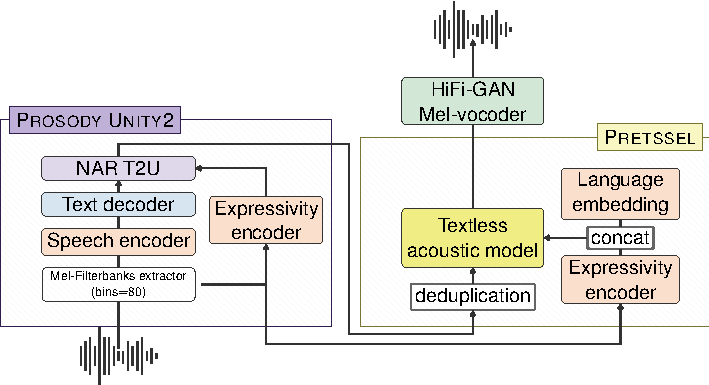
\includegraphics[width=.8\linewidth]{figures/expressivity/seamless_expressive_simplified.pdf}
\caption{\textbf{Overview of \seamlessexpressive.} Model architecture with two main-submodules, \prosodyunitytwo and \ptv.}
\label{fig:expressive:seamless_expressive}
\end{figure}

The proposed \seamlessexpressive translation system, as illustrated in~\Cref{fig:expressive:seamless_expressive}, incorporates \textit{\ptvemb} in both the translation model and speech generator of the \mfourttwo's design. This allows us to maintain high semantic translation quality given by the backbone system. In other words, we propose a cascaded expressive modeling pipeline that consists of two main sub-modules: (1) \prosodyunitytwo, which is a prosody-aware speech-to-unit translation model based on \unitytwo architecture, and (2) \ptv, a novel textless acoustic model featuring cross-lingual expressivity preservation during unit-to-speech generation.

\prosodyunitytwo and \ptv are designed to complement each other in transferring the expressiveness of source language speech.
That means, \prosodyunitytwo aims to transfer phrase-level prosody such as speech rate or pauses, while \ptv transfers utterance-level expressivity like the style of one's voice.
From the following sections, we first introduce \ptv and \prosodyunitytwo architectures and how they can transfer these expressivity aspects from source language to target language speech.
Then, we discuss how both components are used together to give rise to expressive speech-to-speech translation.

\subsubsection{\ptv: Expressive unit-to-speech generator}
\label{sec:p2v}

\begin{figure}[!tbh]
\centering
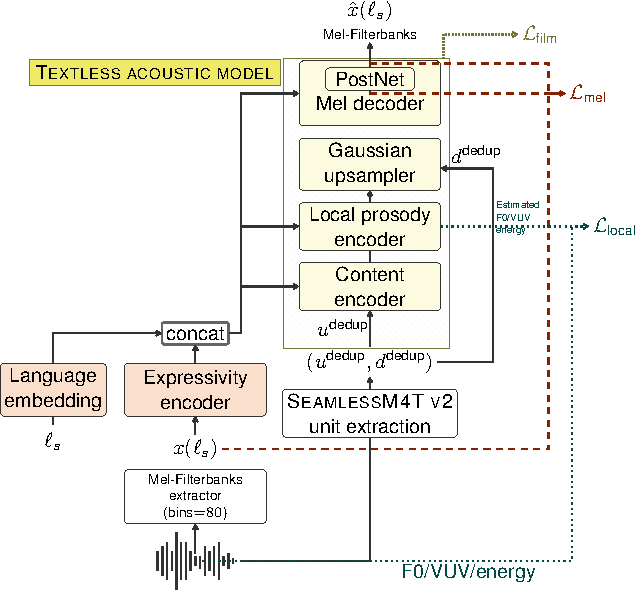
\includegraphics[width=.7\linewidth]{figures/expressivity/p2v.pdf}
\caption{\textbf{\ptv pre-training.} Illustration showing the three loss terms of \Cref{eq:expressive:ptv} used to optimize \ptv's parameters.}
\label{fig:expressive:p2v}
\end{figure}

For the high-quality cross-lingual expressivity transfer, we propose a \textbf{P}aralinguistic \textbf{RE}present\-ation-based \textbf{T}extle\textbf{SS} acoustic mod\textbf{EL}, or \ptv. \ptv can efficiently disentangle semantic and expressivity components from source language speech through unsupervised speech reconstruction pretraining.
The overall architecture of \ptv and its pretraining process are illustrated in \Cref{fig:expressive:p2v}.
More specifically, \ptv was pretrained to reconstruct 80-dimensional Mel-filterbank features of input speech from the deduplicated (or reduced) XLS-R units with 10k k-means clustering and the same Mel-filterbank features.
After pretraining, the model is capable of expressivity-preserving Mel-filterbank generation by taking a unit sequence in the target language and Mel-filterbank features in source speech as the expressive prompt.
Lastly, the HiFi-GAN vocoder~\citep{kong2020hifi} synthesizes speech waveform from the Mel-filterbank features.



The proposed \ptv is composed of \ptvenc that extracts \ptvemb vector from the source language speech and the textless acoustic model that generates the Mel-filterbank features from \ptvemb and the XLS-R units.
We detail each module in the following subsections.

\paragraph{\ptvenchead.}
\label{sec:p2v_enc}
The \ptvenc extracts a 512-dimensional \ptvemb vector containing high-level paralinguistic representations from the input 80-dimensional Mel-filterbank features.
As a backbone network, we adopted a modified version of the ECAPA-TDNN architecture. The choice of the model architecture was motivated by its high performance in extracting speech's acoustic representation~\citep{desplanques-ecapa-tdnn-2020}.
In our model, we replaced the batch normalization layer~\citep{ioffe2015batch} with layer normalization~\citep{lei2016layer} for consistent performance at different batch sizes.
Once \ptvemb is extracted, we normalized it with the L2 norm to make the training process more stable.

Note that the XLS-R units mainly contain linguistic information of speech~\citep{SeamlessM4TArXiv}.
Thus, as mentioned by~\citet{skerry2018towards}, the information that \ptvemb learns becomes paralinguistic information, including prosody information and other acoustic properties such as the style of one's voice.
As a result, when it comes to expressive S2ST, both prosody and vocal style characteristics can be efficiently transferred to output speech by extracting \ptvemb from source language speech.


\paragraph{Textless acoustic model.}
\label{sec:p2v_am}
The textless acoustic model predicts a Mel-filterbank features of output speech for given \ptvemb and XLS-R units.
We adopted a non-autoregressive (NAR) Transformer model derived from FastSpeech2~\citep{ren2021fastspeech2}, where the XLS-R units are used as a linguistic input instead of text or phoneme sequence. %

Specifically, the content encoder first extracts a high-level context representation from XLS-R units using a positional encoding layer followed by feed-forward Transformer (FFT) blocks. 
Then, \ptvenc predicts unit-level local prosody features defined by F0 and energy contours and adds them to the context encoder output.
The Gaussian upsampler proposed by \citet{shen2020nonattentive} is adopted to upsample the unit-level hidden sequence to the frame-level time scale using unit duration.
Mel-decoder then generates the Mel-filterbank features of output speech from an upsampled hidden sequence using a positional encoding layer followed by FFT blocks.
To predict more naturally generated Mel-filterbank features, we used PostNet, proposed by \citet{jonathan2017natural}, to compensate for the residual signal that the decoder's FFT blocks could not capture.

Even though the overall architecture is similar to FastSpeech2, there are clear differences.
First, we actively used \ptvemb and language embedding vectors during the Mel-filterbank generation process for effective language-dependent expressivity transfer.
In particular, inspired by \citet{Za_di_2022}, we applied FiLM conditioning layer \citep{perez2018film, boris2018tadam} for conditioning prosody and language embeddings to every FFT block output and local prosody predictor as:
\begin{align}\label{eq:expressive:film}
    \nonumber \text{film}(h,c) &= (\gamma+1) \cdot h + \beta, \\ 
    \gamma &= f_1(c) \cdot \theta_{\gamma},\\
    \nonumber \beta &= f_2(c) \cdot \theta_{\beta},
\end{align}
where $h,c$ are respectively the hidden representation and the corresponding conditional embedding; $f_1,f_2$ are linear projections and $\theta_{\gamma}, \theta_{\beta}$ are learnable scalar parameters.
The intuition behind this parameterized layer is to adjust the conditional embedding vector given its value relative to the hidden representation at every time step.

Second, instead of predicting the unit duration with the internal local prosody predictor~\citep{ren2021fastspeech2}, we used predicted duration from \unitytwo for its better unit sequence modeling.
For a given unit duration obtained by \unitytwo, we simply converted it to Mel-duration by scaling it by a factor of two, which is the ratio between intervals of Mel-filterbank features (i.e., 10 ms) and unit extraction (i.e., 20 ms).
Then, we used a Gaussian upsampler~\citep{shen2020nonattentive} to upsample unit-scale features to match the Mel-scale features.
Unlike the original Gaussian upsampler that predicts the standard deviation of the Gaussian component, we set it to a constant value $T^2=10$ for simplicity.
As mentioned in \citet{shen2020nonattentive}, this is more similar to the single Gaussian soft monotonic attention compared to the length regulator of FastSpeech2 mimicking hard monotonic attention.
Thus, the upsampled hidden features show continuous transition at the unit boundary, which is more efficient for representing continuously varying target Mel-filterbank features.

We also propose to split the binary voiced/unvoiced (VUV) flag from the F0 contour and separately predict them during the local prosody prediction process.
After predicting continuous F0 contour and binary VUV flag, we combine them by simply masking F0 values at unvoiced regions to zero.
By externally imposing VUV properties during the local prosody encoding process, the model can more distinctively represent VUV properties in its output Mel-filterbank features.

\paragraph{Unsupervised pretraining.}
During pretraining, \ptvenc and textless acoustic model are jointly trained to minimize three loss terms:
\begin{align}
    \mathcal{L}_{total} = \mathcal{L}_{mel} + \lambda_{l} \cdot \mathcal{L}_{local} + \lambda_{f} \cdot \mathcal{L}_{film},\label{eq:expressive:ptv}
\end{align}
where $\mathcal{L}_{mel}$, $\mathcal{L}_{local}$, and $\mathcal{L}_{film}$ denote Mel-filterbank prediction loss, local prosody prediction loss, and L2 regularization loss at the FiLM layer, respectively; $\lambda_{v}$ and $\lambda_{v}$ denote weight terms for $\mathcal{L}_{local}$ and $\mathcal{L}_{film}$ that are set to be $1.0$ and $0.001$, respectively.
Each term is formulated as follows:
\begin{align}
    \mathcal{L}_{mel} &= \mathcal{L}_1(\hat{{y}}_{before}, {y}) + \mathcal{L}_2(\hat{{y}}_{before}, {y}) + \mathcal{L}_1(\hat{{y}}_{after}, {y}) + \mathcal{L}_2(\hat{{y}}_{after}, {y}), \\
    \mathcal{L}_{local} &= \mathcal{L}_2(\hat{{p}}, {p}) + \text{BCE}(\hat{{u}}, {u}) + \mathcal{L}_2(\hat{{e}}, {e}), \\
    \mathcal{L}_{film} &= \sum_{\theta_{\gamma},\theta_{\beta}}\left(\theta_{\gamma}^2 + \theta_{\beta}^2\right),
\end{align}
where $\mathcal{L}_1(\cdot, \cdot)$, $\mathcal{L}_2(\cdot, \cdot)$ and $\text{BCE}(\cdot, \cdot)$ denote L1, L2, and binary cross-entropy losses, respectively; $\hat{{y}}$ and ${y}$ denote predicted and reference Mel-filterbank features, respectively; $before$ and $after$ subscripts imply the one before and after PostNet, respectively; ${p}$, ${e}$, and ${u}$ denote log-scale pitch contour where its unvoiced region is linearly interpolated, log-scale energy, and VUV flag, respectively.
We involve $\mathcal{L}_{film}$ for better generalization performance of the textless acoustic model as reported in \citet{boris2018tadam}.
Note that each loss term does not require any text transcriptions or human data annotations, and it is easily scalable to large-scale data and more language directions.

\paragraph{Relationship to prior works.}
 The key difference of \ptv-based expressive S2ST system compared to \mfourttwo is that it utilizes source language's \ptvemb during the speech generation process.
The unit-based HiFi-GAN for \mfourttwo reconstructs speech waveform from XLSR-R units and language embedding without any connection to expressivity information.
Thus, it tends to produce monotone speech in terms of vocal style and prosody.
In contrast, the proposed \ptv overcomes this limitation by explicitly conditioning source language's \ptvemb.

A work similar to \ptv is the \textsc{Prosody2Vec} framework~\citep{qu2022disentangling}. %
It similarly proposed a textless acoustic model based on Tacotron2~\citep{jonathan2017natural} by replacing phoneme input with HuBERT units~\citep{hsu2021hubert}.
The major differences between our effort and \textsc{Prosody2vec} are: (1) we adopted NAR FastSpeech2-based acoustic model for fast inference, (2) we integrated this model into expressive S2ST system, and (3) we adopted XLS-R units for the easy language scalability.

On the other hand, the \textsc{PolyVoice}~\citep{polyvoice} also adopted a similar cascaded approach for expressive S2ST by incorporating cascaded language models (LMs) at speech-to-unit translation and unit-to-speech generation modules.
In particular, it uses hybrid AR and NAR LM to generate SoundStream units~\citep{Zeghidour2022SoundStreamAE} at target language from the target language's HuBERT units and the source language's SoundStream units. 
Despite its high-quality expressive translation, \ptv has strong benefits considering hybrid AR and NAR LM's lower inference speed.
Even though \unitvb described in~\Cref{sec:expressive:unit_voicebox} can be a good alternative as an NAR unit-to-speech generator, it still lags inference speed compared with \ptv because its architecture requires heavier model size.
More analysis is included in~\Cref{subsec:express_exp}.






\subsubsection{\prosodyunitytwo: Expressive speech-to-unit translation model}

\begin{figure}[!tbh]
\centering
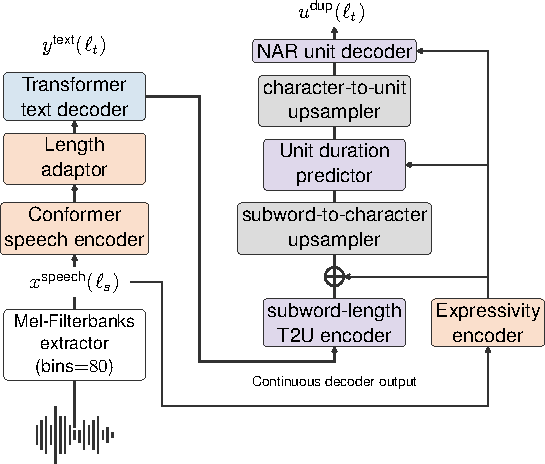
\includegraphics[width=.6\linewidth]{figures/expressivity/prosody_unity2.pdf}
\caption{\textbf{\prosodyunitytwo.} Illustration of modules building on \unitytwo.
}
\label{fig:expressive:prosody-unity2}
\end{figure}

For the expressive speech-to-unit translation, we propose a \prosodyunitytwo, which incorporates \ptv's \ptvemb during the unit generation process. As illustrated in \Cref{fig:expressive:prosody-unity2}, the proposed \prosodyunitytwo is based on UnitY2's architecture that takes Mel-filterbank features of source language speech as input, and outputs 20-ms interval XLS-R 10K units of target language speech.


\paragraph{Prosody-aware NAR T2U architecture.}

To better transfer expressivity information of source speech during the unit generation process, \prosodyunitytwo injects \ptvemb extracted by \ptvenc from the source speech into various positions of NAR T2U component: (1) adding \ptvemb to the output of subword-length T2U encoder, and (2) conditioning the unit duration predictor and NAR unit decoder on the transformed \ptvemb by a FiLM layer, as described in \Cref{eq:expressive:film}.


Components in \unitytwo, such as the duration predictor and NAR unit decoder, are capable of word/phrase-level prosody modeling concerning pauses and speech rate. However, it remains a non-trivial task for \unitytwo to preserve them because its T2U component does not predict units explicitly conditioned on acoustic information from source speech. 
The proposed prosody-aware T2U component can effectively address this limitation by integrating \ptvemb into unit prediction.

\paragraph{Fine-tuning pretrained components.}
We used the \st model described in~\Cref{sec:offline:x2t} as the foundation model and deployed it to initialize the speech encoder and the first-pass text decoder of \prosodyunitytwo.
The MAdaptor layer of the \st component of \prosodyunitytwo is initialized using the GeLU activation function (where the original model uses ReLU), allowing the model to avoid quick overfitting during finetuning. In contrast to the training design of \Cref{sec:offline:s2st}, we finetuned the parameters of the \st component so that the text decoder is able to learn pause labels located in our text training data.

In addition, for efficient prosody-aware training, we initialized \ptvenc from the parameters of the pretrained \ptv.
Then, all model parameters, including \st and \ptvenc, were jointly trained to optimize conventional \unitytwo training criteria, as explained in~\Cref{sec:offline:unity2_training}.



\subsubsection{Expressive S2ST with \seamlessexpressive}
As illustrated in \Cref{fig:expressive:seamless_expressive}, we separately trained \prosodyunitytwo and \ptv and constructed the proposed \seamlessexpressive by cascading the two components.
During inference, \prosodyunitytwo translates source speech into XLS-R units of target language conditioned by \ptvemb.
Given unit duration and reduced units, the textless acoustic model of \ptv synthesizes the Mel-filterbank features of target language speech from XLS-R units.
Specifically, the concatenated vector of the source language's \ptvemb and the target language's language embedding are used as the conditional vector of the acoustic model.
Finally, the HiFi-GAN vocoder~\citep{kong2020hifi} converts Mel-filterbank features into the speech waveform.


\subsection{Experimental Setup}

\begin{table}
    \centering
    \begin{tabular}{lrrrrrr}
    \toprule
        \textbf{Set} & \textbf{cmn}       & \textbf{deu}       & \textbf{eng}       & \textbf{fra}       & \textbf{ita}   & \textbf{spa}  \\ \midrule
      Training & 12,771 & 1,965  & 44,571 & 1,073  & 247  & 915  \\
      Validation   &  20   &   14   &  16    &  10     & 5  &  10  \\
    \bottomrule
    \end{tabular}
    \caption{\textbf{\ptv data statistics.} Duration in hours of \ptv pretraining datasets per language.}
    \label{tab:ptv_pretrain_data}
\end{table}

\paragraph{\ptv.}
To train \ptv, we extracted 80-dimensional Mel-filterbank features and 10K XLS-R units using the same methods as \mfourttwo.
Then, we applied zero-mean and unit-variance normalization to input and output Mel-filterbank features to stabilize model training.

To extract F0 and VUV flag, we first extracted F0 in every 5 ms by using DIO algorithm~\citep{morise2016world}.
Then, we obtained VUV flag specifying non-zero values of F0, while obtaining continuous F0 contour by linearly interpolating zero values.
To extract energy, we extracted energy contour every 5 ms using a 35-ms Hanning window.
Using the duration of unit, all F0, VUV flag, and energy features were averaged to have a reduced unit-scale.
Finally, we converted linear F0 and energy values into log-scale.

At the pretraining stage, we collected several multilingual datasets covering six languages described at~\Cref{sec:expressive_data}. 
We summarize the data statistics in \Cref{tab:ptv_pretrain_data}.
To alleviate language imbalance in training data, we applied temperature-based resampling with the temperature set to 5.
For better generalization of \ptvemb, SpecAugment~\citep{park2019specaugment} with frequency mask with a maximum width of 8 and time mask with a maximum width of 10 was applied on the fly during training.
The \ptv model was trained by $500$k iteration using 16 V100 GPUs with a learning rate of $10^{-4}$.


We randomly sampled 10k utterances from each language of \ptv training data.
and trained a HiFi-GAN model~\citep{kong2020hifi} for one million iterations with a fixed batch size of 16, batch length of 8,960, and 8 V100 GPUs.
We modified the original HiFi-GAN's upsampling scales from [8, 8, 2, 2] to [5, 4, 4, 2] because the Mel-filterbank features's 10-ms frame interval equals 160 samples.
We further fine-tuned the HiFi-GAN vocoder by using the output of the \ptv for 400k iterations to prevent the quality degradation from over-smoothing problem~\citep{bishop94mixturedensity}.
Specifically, we generated over-smoothed Mel-filterbank features by inference \ptv under teacher-forcing mode to prepare a pair of Mel-filterbank features and waveform for fine-tuning.
All other training settings follow the original HiFi-GAN training setup~\citep{kong2020hifi}.








\unitvb is pre-trained on the data in \Cref{tab:ptv_pretrain_data} as \ptv. We include a baseline S2ST system with \ptv as the acoustic model (see Model 4 in \Cref{tab:expressive_models}) to compare with \ptv in speech synthesis. For data preprocessing introduced in \Cref{sec:expressive_data}, we further finetune \unitvb on emotional data to synthesize diverse speech. We describe more pre-training and finetuning details in the Appendix.

\begin{table}[htp!]
    \centering
    \small
    \begin{tabular}{rccccc}
        \toprule
         & \begin{tabular}{@{}c@{}} \textbf{Expressive} \\ \textbf{Alignments} \end{tabular} &  \begin{tabular}{@{}c@{}} \textbf{\sonar} \\ \textbf{Expressive} \end{tabular} &  \begin{tabular}{@{}c@{}} \textbf{Video} \\ \textbf{Alignments} \end{tabular} &  \textbf{Commissioned} &  \textbf{cTTS}\\
        \midrule
        French & 1,949 & 646 & 299 & 0 & 1,515 \\ 
        German & 994 & 662 & 122 & 17 & 1,503 \\
        Italian & 286 & 688 & 68 & 18 & 1,614 \\ 
        Mandarin & 110 & 42 & 286 & 14 & 1,402 \\ 
        Spanish & 1,729 & 866 & 237 & 31 & 1,637 \\ 
        \midrule
        \textbf{Total} & 5,068 & 2,904 & 1,012 & 80 & 7,671 \\
        \bottomrule
    \end{tabular}
    \caption{\textbf{\prosodyunitytwo data statistics.} Number of source speech hours in training data per data source and language direction.
    }
    \label{tab:expressivity-training-hours-per-dataset}
\end{table}

\paragraph{\prosodyunitytwo.} We combined data from all training data sources and language directions described in \Cref{tab:expressivity-training-hours-per-dataset}.
Given the large amount of \sonar data,%
we set thresholds and filtered the high-quality data:
for \sonar data, we selected source-target pairs with \comparator scores greater or equal to~3.2 and cosine scores greater or equal to~0.75 for all directions. The amount of other data sources used for training is the same as reported in \Cref{tab:expressivity-num-hours-per-dataset}.
With training data in $10$ directions between English and five languages, we trained a single multilingual speech-to-unit translation model for conducting objective evaluation with automatic metrics and subjective human evaluation (\Cref{sec:humaneval}).
For the ablation study, we trained five bidirectional models for each language pair (\xeng and \engx), one eng-to-many (E2M) model, and one many-to-eng (M2E) model. Those models help us understand how multilingual training affects translation performance.

All models were trained with a learning rate of $5\times10^{-5}$. 
Bidirectional and M2E models were trained in a distributed setup with an effective batch size of 302k tokens; E2M and M2M have a larger batch size of $360$k tokens. We set a maximum of $600$k training steps and adopted an early stop policy such that model training is stopped when validation loss has not been improved for the last $5$ runs. The checkpoint with the best validation loss is used for evaluation.




\paragraph{Automatic metrics.} We adopted the following automatic metrics to measure both the semantics and the expressive aspects of \seamlessexpressive.
\begin{itemize}
    \item \asrbleu. Our expressive translation systems must maintain high-quality content translation. We do model selection and analysis using average \bleu for \st and \asrbleu for \sst (see \Cref{tab:metrics}). 
    This pair of scores allows us to see the final model performance and how much the translation quality alters between text and its audio realization.
    \item Vocal style similarity (VSim). Embeddings are extracted from generated and source speech using a pretrained WavLM-based encoder \citep{wavlm}. We measured the cosine similarity of the embeddings (as in Voicebox \citep{le2023voicebox}).
    \item \comparator score. 
    For sentence-level prosody transfer, we relied on the \comparator model trained on multilingual data (see \Cref{sec:comparator} for more details). 
    \item Rhythm: speech rate Spearman correlation (Rate) and joint pause alignment score (Pause). Speech rate is estimated from source and generated speech as described in \Cref{sec:expressivity_metrics}, and we report Spearman correlation between the rates of the source and the target. Pause preservation was measured using the weighted mean joint pause alignment score from the rhythm evaluation toolkit described in \Cref{sec:local-prosody-tools}.
\end{itemize}






\subsection{Results and Discussion}
\label{subsec:express_exp}

In this section, we trained \seamlessexpressive models for expressive speech-to-speech translation. A card for these models is available in \Cref{card:seamlessexpress}. We also perform empirical evaluation on \seamlessexpressive models together with different baselines, and $10$ translation directions are included: 
English$\leftrightarrow$\{French (fra), German (deu), Italian (ita), Mandarin (cmn), Spanish (spa)\}.

\paragraph{Models.} \Cref{tab:expressive_models} summarizes the model list for expressive S2ST evaluation. Given current progress in vocal style-preserved text-to-speech such as \coqui\footnote{\url{https://huggingface.co/coqui/XTTS-v2}}, we included a strong cascaded baseline, Model 1, which consists of speech-to-text modules in \mfourttwo and the text-to-speech model \coqui.

Our proposed model is Model 5, \seamlessexpressive trained with 5-eng and eng-5 translation data. A natural baseline is Model 2, \mfourttwo, which serves as our foundational model. To analyze the performance of \ptv, Model 3, which replaced the unit HiFi-GAN in \mfourttwo with \ptv, is included as another baseline to measure the effectiveness of \prosodyunitytwo when compared against Model 5 and evaluates \ptv in comparison with Model 2. 

As \unitvb is able to convert units to speech and is also used for training data augmentation, we introduced Model 4 to compare \ptv with \unitvb in speech generation. For a fair comparison with \ptv, the pretrained checkpoint of \unitvb is used in Model 4, and the finetuned \unitvb is only for the purpose of data augmentation. 




\begin{table}[htbp!]
    \small
    \centering
    \begin{tabular}{cccc}
    \toprule
       \textbf{ID}  & \textbf{Model} & \textbf{ Speech-to-Unit/Text} &  \textbf{Unit/Text-to-Speech}  \\ \midrule
        1 & \st+\tts & \mfourttwo \st & \coqui \\
        2  & \mfourttwo & \unitytwo & Unit HiFi-GAN  \\
        3  & - & \unitytwo & \ptv \\
        4  & - & \prosodyunitytwo & \unitvb  \\
        5 (proposed)  & \seamlessexpressive & \prosodyunitytwo & \ptv \\ \bottomrule
    \end{tabular}
    \caption{\textbf{List of models for expressive \sst.} Model 1 uses text outputs from \st to synthesize speech, and Model 2-5 connect speech-to-unit and unit-to-speech components with predicted units.}
    \label{tab:expressive_models}
\end{table}



\paragraph{Evaluation data.} We prepared three evaluation sets of expressive speech-to-speech translation in mExpresso, mDRAL (\Cref{sec:expressive_data})\footnote{We will release the benchmark sets.} and FLEURS. The data statistics of dev and test splits are reported in \Cref{tab:expressive_dev_test_data}.

\begin{table}[htbp!]
    \small
    \centering
    \begin{tabular}{lrrrrrr}
        \toprule
         & \multicolumn{2}{c}{\textbf{mExpresso}} & \multicolumn{2}{c}{\textbf{mDRAL}} & \multicolumn{2}{c}{\textbf{FLEURS}}  \\ \cmidrule(r){2-3}\cmidrule(lr){4-5}\cmidrule(l){6-7}
         & Dev & Test & Dev & Test & Dev & Test \\ \midrule
        Sample \#              & 25520 &  33694  & 2715 & 2293 & 3784 & 7438  \\
        Hours                  & 28.96 & 39.67   & 5.42 & 5.16 & 11.31  & 23.50 \\
        Total \# Speakers      & 11    & 12      & 53 & 55 & - & - \\
        Total \# Male Speakers & 5     & 6       & 18    & 19 & -  & - \\
         \hline
    \end{tabular}
    \caption{\textbf{Descriptive statistics of evaluation data}. Statistics of the development (dev) and test splits of mExpresso, mDRAL and \fleurs. Note that we do not have speaker information for \fleurs so these rows are left empty. Since the mExpresso dataset is pivoted out of English, to avoid double counting English volumes we only include the unique English samples in these descriptive statistics (along with the other languages).   \Cref{tab:expressive_dev_test_data_lang_pair_level} provides these descriptive statistics for each language pair.}
    \label{tab:expressive_dev_test_data}
\end{table}







\begin{table}
    \centering
    \begin{tabular}{cccccc}
        \toprule
        & \textbf{Model} & $\uparrow$\textbf{\asrbleu} & $\uparrow$\textbf{\comparator} & $\uparrow$\textbf{Rate} \\
        \midrule
        \multirow{5}{*}{\begin{tabular}[c]{@{}l@{}}\xeng\\ $(n=5)$ \end{tabular}} & 1 & 31.95 & 2.83 & 0.35 \\
        & 2 & 34.47 & 2.16 & 0.08 \\
        & 3 & 34.27 & 2.76 & 0.27 \\
        & 4 & \textbf{39.27} & 3.14 & \textbf{0.64} \\
        & 5 & 39.00 & \textbf{3.18 }& 0.63 \\
        \midrule
        \multirow{5}{*}{\begin{tabular}[c]{@{}l@{}}\engx \\ $(n=5)$  \end{tabular}} & 1 & 28.69 & 2.87 & 0.39 \\
        & 2 & 30.35 & 2.44 & 0.09 \\
        & 3 & 30.07 & 2.93 & 0.29 \\
        & 4 & \textbf{34.38 }& \textbf{3.17 }& \textbf{0.65} \\
        & 5 & 34.21 & 3.11 & \textbf{0.65 }\\
        \bottomrule
    \end{tabular}
    \caption{\textbf{Result on mExpresso test data.} Models are compared on \asrbleu, \comparator and Rate metrics, and we exclude VSim and Pause as mExpresso is acted short speech with only one or two speakers per set.
    }
    \label{tab:express_main_results_mexpresso}
\end{table}

\begin{table}
    \centering
    \begin{tabular}{ccccccc}
        \toprule
        & \textbf{Model} & $\uparrow$\textbf{\asrbleu} & $\uparrow$\textbf{VSim} & $\uparrow$\textbf{\comparator} & $\uparrow$\textbf{Rate} & $\uparrow$\textbf{Pause} \\
        \midrule
        \multirow{5}{*}{\begin{tabular}[c]{@{}l@{}}\xeng\\ $(n=5)$ \end{tabular}} & 1 & 36.69 & 0.33 & 2.78 & 0.24 & 0.26 \\
        & 2 & 38.82 & 0.05 & 2.31 & 0.13 & 0.14 \\
        & 3 & 38.59 & 0.27 & 2.87 & 0.15 & 0.16 \\
        & 4 & 40.13 & \textbf{0.36} & 3.13 & 0.63 & \textbf{0.39} \\
        & 5 & \textbf{40.18 }& 0.28 & \textbf{3.19} &\textbf{ 0.64} & \textbf{0.39} \\
        \midrule
        \multirow{5}{*}{\begin{tabular}[c]{@{}l@{}}\engx \\ $(n=5)$  \end{tabular}} & 1 & 23.63 & 0.39 & 2.61 & 0.21 & 0.21\\
        & 2 & 25.32 & 0.06 & 2.36 & 0.06 & 0.14 \\
        & 3 & 24.75 & 0.33 & 2.76 & 0.09 & 0.14 \\
        & 4 & \textbf{34.13} & \textbf{0.40 }& \textbf{2.92} & 0.58 & 0.35 \\
        & 5 & 33.82 & 0.33 & \textbf{2.92} & \textbf{0.59 }& \textbf{0.36} \\
        \bottomrule
    \end{tabular}
    \caption{\textbf{Result on mDRAL test data.} All evaluation metrics are reported as mDRAL is spontaneous expressive speech which is useful for comparing different aspects of prosody.
    }
    \label{tab:express_main_results_mdral}
\end{table}


\begin{table}
    \centering
    \begin{tabular}{ccc}
         \toprule
         & \multicolumn{2}{c}{$\uparrow${\textbf{\asrbleu}}} \\\cmidrule(rr){2-3}
        Model & \makecell[c]{\xeng \\ $(n=5)$} & \makecell[c]{\engx\\ $(n=5)$ }\\
        \midrule
        1 & 31.34 & 16.59 \\
        2 & \textbf{31.99 }& \textbf{31.78} \\
        3 & 31.81 & 29.28 \\
        4 & 30.58 & 31.58 \\
        5 & 30.47 & 29.32 \\
        \bottomrule
    \end{tabular}
    \caption{\textbf{Results on FLEURS test data.} Model are compared on \asrbleu only as FLEURS is commonly used to evaluate content preservation in translation.
    }
    \label{tab:express_main_results_fleurs}
\end{table}





\paragraph{Metric comparison.} We empirically evaluated models using both dev and test splits of multiple datasets. Covering multiple evaluation metrics, average results\footnote{{Watermarking is applied to released models, so they might have slight difference with reported results in the paper.}} are reported over five \xeng and five \engx directions, respectively. \Cref{tab:express_main_results_mexpresso} reports test results on mExpresso, \Cref{tab:express_main_results_mdral} on mDRAL, and \Cref{tab:express_main_results_fleurs} on FLEURS. These datasets represent different aspects of systems' performance we focus on. Both mDRAL and mExpresso involve explicit expressivity alignment, thus allowing us to monitor \comparator score for sentence-level prosody alignment and speech rate, and mDRAL contains spontaneous speech with natural pauses for us to evaluate the quality of pause preservation. FLEURS is mostly used to examine how the model is maintaining content translation quality from \mfourttwo.

More detailed results in each language direction can be found in the appendix, where \Cref{tab:express_mexpresso} reports results on mExpresso, \Cref{tab:express_mdral} on mDRAL, and \Cref{tab:express_fleurs} on FLEURS data. In this section,
we focus on comparing the models' performance on test sets because all conclusions we make also hold on development sets.
    \paragraph{Expressive speech-to-unit translation.} 
    We compare \prosodyunitytwo and \unitytwo by looking at Models 5 and 3, which differ in the speech-to-unit module. Model 5 demonstrates competitive \asrbleu. Averaged over five \xeng directions, the gains of Model 5 on test data are +$4.73$ BLEU in mExpresso and +$1.59$ BLEU in mDRAL while falling behind Model 3 by $1.34$ BLEU in FLEURS. The average gains in five \engx directions are +$4.14$ and +$9.07$ BLEU on mExpresso and mDRAL test sets, respectively. Both models have comparable \asrbleu in FLEURS \engx data.
    \paragraph{Expressive speech generator.}The comparison of Model 3 against Model 2 reflects the effectiveness of \ptv. Models 3 and 2 are close in terms of rate and pause metrics across three datasets, as these aspects are mainly controlled by the speech-to-unit translation model.
    \ptv makes good improvements in preserving prosody and the style of one's voice in generated speech. Given mDRAL test data in \Cref{tab:express_main_results_mdral}, \ptv yields +$0.22$ vocal style similarity and +$0.56$ \comparator in \xeng translations, +$0.27$ vocal style similarity and +$0.4$ \comparator in \engx translations. Both models have similar \asrbleu, indicating that the preserved expressivity did not severely degrade the intelligibility of the output audio.

\begin{figure}
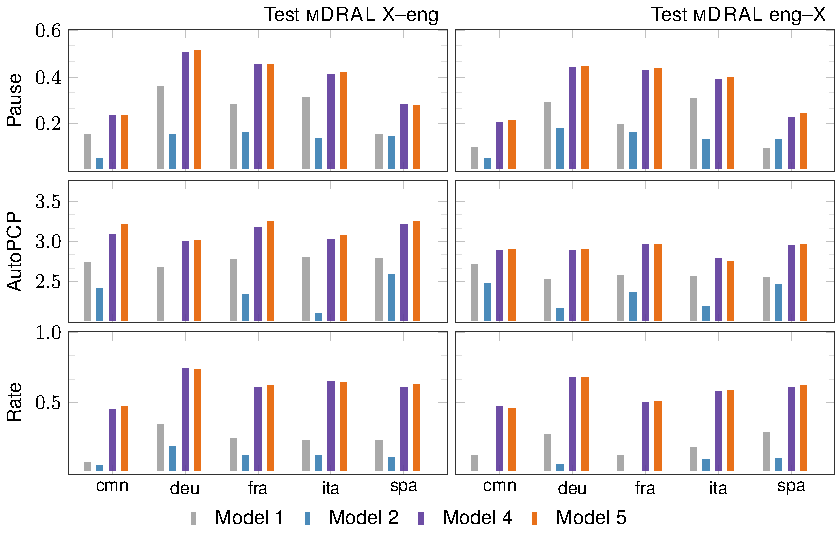
\includegraphics[width=.9\linewidth]{figures/expressivity/expressivity_barplots_new.pdf}
\caption{\textbf{Language-specific \sst performance.} Evaluation results of speech-to-speech translation systems with the focus on newly proposed automatic metrics and measured on mDRAL set.}
\label{fig:expr_barplots}
\end{figure}
    
    \paragraph{Combining into \seamlessexpressive.} Combining the strengths of \prosodyunitytwo and \ptv, \seamlessexpressive (Model 5) demonstrates not only improved content translation but also better preservation of rhythm, tone, and the style of one's voice over the baseline \mfourttwo (Model 2).
    \Cref{fig:expr_barplots} further focuses on prosody-related metrics (Pause, Rate, \comparator) and breaks down the performance of each language measured on mDRAL test data, where we see consistent improvement across different language directions.
    
    
    \paragraph{Alternative expressive speech generator} We examine using \unitvb as an alternative option for expressive speech generation. We note that \unitvb, with $329$M parameters, is a much larger model than \ptv with $65$M parameters. Furthermore, \ptv is faster in speech synthesis: the real-time factor (RTF) of \ptv is $0.014$ and $0.089$ for \unitvb. Given the 6x lower RTF, \ptv is a better fit as a speech generator considering the model size and inference efficiency when we equip \seamlessexpressive with streaming capability in \Cref{sec:unified}. Models 5 and 4 show that the speech generator choice mainly results in a trade-off in vocal style similarity (with \unitvb having higher vocal style similarity), while the performance in \comparator is similar across different language pairs (\Cref{fig:expr_barplots}).
    \paragraph{Expressive \st+\tts cascade} We observe that the strong cross-lingual vocal styles and style-preserving \tts system is sensitive to the noise in the source speech, resulting in a much lower \asrbleu than \seamlessexpressive, which is the most fundamental metric of an \sst system. The \tts system is better in preserving the source speakers' vocal styles, while \seamlessexpressive outperforms in prosody preservation with consistent gains on \comparator, speech rate, and pause metrics across language directions (\Cref{fig:expr_barplots}).


\subsection{Ablation Study}
We conducted ablation experiments to study the effectiveness of different training data and modeling choices.
We focused on mDRAL for the ablation studies as it allows us to examine all the semantic and prosodic metrics meaningfully. 

\subsubsection{Data ablation}
We validated the effectiveness of all data sources listed in \Cref{tab:expressivity-training-hours-per-dataset} on \seamlessexpressive by ablating each of them from training with a leave-one-out approach, with results presented in \Cref{tab:expressive_source_ablate}.
We see the major effect of the data sources is on \asrbleu. A large amount of parallel training data helps achieve high content translation quality, while the prosody preservation performance can be maintained due to prosody-aligned parallel datasets.


\begin{table}[htbp!]
    \centering
    \setlength{\tabcolsep}{4pt} %
    \begin{tabular}{lccccc}
        \toprule
         & $\uparrow$\textbf{\asrbleu} & $\uparrow$\textbf{VSim} & $\uparrow$\textbf{\comparator} & $\uparrow$\textbf{Rate} & $\uparrow$\textbf{Pause} \\ \midrule
        All data         & 54.35 & 0.27 & 3.28 & 0.64 & 0.63 \\
        w/o Commissioned & 53.09 & 0.26 & 3.25 & 0.64 & 0.64 \\
        w/o Video Alignments & 53.11 & 0.27 & 3.26 & 0.64 & 0.61 \\
        w/o cTTS         & 52.60 & 0.26 & 3.27 & 0.60 & 0.59 \\
        w/o \sonar Expressive       & 54.30 & 0.27 & 3.25 & 0.61 & 0.59 \\
        w/o Expressive Alignments       & 53.54 & 0.27 & 3.28 & 0.66 & 0.63 \\
         \bottomrule
    \end{tabular}
    \caption{\textbf{Data source ablation}. Results on unidirectional spa-eng mDRAL test set.}
    \label{tab:expressive_source_ablate}
\end{table}




\subsubsection{Semantic and prosodic data filtering}
\label{subsec:express_data_ablation}
The quality of collected expressive data is variable. 
Some segments may contain different semantic content, harmful for translation, while others may evince similar content but with different prosody, harmful for expressive translation.
With this idea in mind, we conducted an analysis to better understand how to characterize and filter data based on their relevance for training an expressive translation system.
For the sake of time, the ablation study described below is conducted only on video-aligned data. We chose this dataset because it is very rich (and also noisy) in terms of both semantic and prosody.

\paragraph{Semantic analysis.}

The data is split into three equal-sized parts, one for each semantic quality, i.e., high, medium, and low semantic score. 
The semantic score of a sample is a mixture of several semantic scores:
\begin{itemize}
    \item BLASER speech similarity,
    \item cosine similarity between source and target text embeddings, and
    \item cosine similarity between source and target speech embeddings.
\end{itemize}

\noindent Model 5, \seamlessexpressive, is then finetuned with each data split, all other parameters unchanged, and then evaluated (see \Cref{tab:sem_pro_ablation_results}).


\paragraph{Prosody analysis: the case of speech rate.}

Another important aspect of training an expressive speech translation model is the prosodic quality of the training data.
To evaluate the finetuning data's impact, we analyzed the expressive training data and trained several models to contrast the results.
For the sake of simplicity, we only considered speech rate in this study, but we evaluated all semantic and prosodic scores.

To compare the speech rates of several languages, it is important to take their relative differences into account since some languages are naturally uttered faster than others.
Thus, we first normalized the speech rate of audio files in a language by the mean for that language and calculated the relative difference between source and target normalized speech rates, by dividing by their average, as follows:
\begin{align}
\textrm{SRD}_\text{norm}(\textrm{S}_{L1}, \textrm{S}_{L2}) = \frac{\textrm{SR}_\text{norm}(\textrm{S}_{L1}) - \textrm{SR}_\text{norm}(\textrm{S}_{L2})}{\textrm{SR}_\text{norm}(\textrm{S}_{L1}) + \textrm{SR}_\text{norm}(\textrm{S}_{L2})},
\end{align}
where $\textrm{S}_{Lx}$ is a segment in language $Lx$, $\textrm{SR}_\text{norm}$ is the normalized speech rate of $\textrm{S}_{Lx}$, and $\textrm{SRD}_\text{norm}$ is the relative speech rate difference.

This measure is then used to split the data into three parts of equal size, similar to what was done for the semantic analysis.
By doing this, we hoped to train systems that better model the relative speech rate difference without considering intra-language variance.
It is worth noting that by looking at the data, we realized that the data labeled as ``semantic/low'' added too much noise to the statistics and that removing them before performing the prosodic analysis was beneficial. 
This means that the three prosodic splits are taken from the high and medium semantic quality data samples only.


\paragraph{Ablation results with semantic and prosodic filtering.}




\begin{table}[hbtp!]
    \centering
\begin{tabular}{cccccccc}
\toprule
 & \textbf{Study} & \textbf{Quality} & $\uparrow$\textbf{\asrbleu} & $\uparrow$\textbf{VSim} & $\uparrow$\textbf{\comparator} & $\uparrow$\textbf{Rate} & $\uparrow$\textbf{Pause} \\
\midrule
\MR{6}{*}{\begin{tabular}[c]{@{}l@{}}\xeng\\ $(n=5)$ \end{tabular}} & \MR{3}{*}{Semantic}  & Low      & 32.15 & 0.26 & 3.09 & 0.62 & 0.25 \\
                    & & Medium   & 35.40 & 0.27 & 3.12 & 0.64 & 0.20 \\
                    & & High     & \bf 40.19 & 0.27 & 3.14 & 0.59 & 0.27\\
\cmidrule{2-8}
& \MR{3}{*}{Prosody}   & Low      & 38.90 & 0.27 & 3.10 & 0.50 & 0.16\\
                    & & Medium   & \bf 39.61 & 0.27 & 3.18 & 0.62 & \bf 0.45\\
                    & & High     & 39.06 & 0.27 & 3.18 & 0.66 & \bf 0.44\\
\midrule
\MR{6}{*}{\begin{tabular}[c]{@{}l@{}}\engx\\ $(n=5)$ \end{tabular}} & \MR{3}{*}{Semantic}  & Low      & 22.56 & 0.31 & 2.84 & 0.51 & 0.13 \\
                    & & Medium   & 28.19 & 0.32 & 2.88 & 0.56 & 0.11 \\
                    & & High     & \bf 33.48 & 0.32 & 2.84 & 0.54 & 0.17 \\
\cmidrule{2-8}
& \MR{3}{*}{Prosody}   & Low      & 32.57 & 0.32 & 2.83 & 0.49 & 0.10 \\
                    & & Medium   & 32.96 & 0.33 & 2.88 & 0.57 & \bf 0.33 \\
                    & & High     & \bf 33.48 & 0.32 & 2.90 & \bf 0.63 & \bf 0.31 \\
\bottomrule
\end{tabular}
\caption{Results of data filtering based on semantic and prosody alignment quality on mDRAL test sets.}
    \label{tab:sem_pro_ablation_results}
\end{table}









\Cref{tab:sem_pro_ablation_results} shows the results of finetuning the model with the semantic and prosodic splits of video data for \xeng and \engx languages pairs, respectively.
Note that the results may not improve upon the baseline system (Model 5, \seamlessexpressive) since we only use the multilingual video data in this study while the baseline model was trained on much more expressive data. 
The comparison of the finetuning results with the three data splits allows us to draw conclusions on the qualitative aspects of the selected data.

Let us first look at the semantic study results. The performance gain is consistent across all datasets and language pairs (see \cref{app:sem_pro_ablation} for language-level breakdown).
We clearly see that the high and medium semantic quality data leads to better \asrbleu scores, with an increase of up to 8\% between \emph{semantic/high} and \emph{semantic/low} setups. 
This motivated us to keep only the average and high semantic quality data splits for the prosodic study.
However, models trained with the semantic splits do not necessarily exhibit better prosodic metric scores.

Looking at the results obtained by finetuning the baseline model with prosodic splits, we observe consistent improvements in speech rate and pause evaluation, which is expected.
By selecting data according to a prosodic criterion (speech rate in our case), we observe improvements in the prosody metrics without hurting the semantic score (\asrbleu) (and sometimes slightly improving it).
This makes sense as it tends to confirm that both aspects are correlated and that segments having the same prosody are more prone to be semantically parallel.
We can also notice that the vocal style similarity metric is not sensitive to the data refinement and remains stable in all our experiments, since it is mainly controlled by the speech generator.

The results are also consistent across language directions (\engx and \xeng) and show that all the considered languages can benefit from selecting higher semantic and prosodic quality data.
Those good results suggest that a better expressive model could be trained by carefully selecting the expressive data from all corpora before finetuning the model. We note that models reported in \Cref{subsec:express_exp} and \Cref{sec:human_eval_test_sets} have not applied such filtering to the training data due to time limit, so we leave that for future work.

\subsubsection{Training ablation}


\begin{table}
    \centering
    \setlength{\tabcolsep}{4pt} %
    \begin{tabular}{cccccc}
    \toprule
       & $\uparrow$\textbf{\asrbleu} & $\uparrow$\textbf{VSim} & $\uparrow$\textbf{\comparator} & $\uparrow$\textbf{Rate} & $\uparrow$\textbf{Pause} \\ \midrule
      \textsc{M2E} & 39.58 & 0.28 & 3.20 & 0.64 & 0.39 \\
      \textsc{M2E-Joint} & 39.02 & 0.18 & 2.92 & 0.65 & 0.36 \\ \midrule
    \end{tabular}
    \caption{Results of jointly trained \seamlessexpressive on mDRAL \xeng test sets. } %
    \label{tab:expressive_joint_results}
\end{table}

\paragraph{Joint training.}

While our main results come from the cascade of \prosodyunitytwo and \ptv models trained separately, we also explored joint training of the two components with the same initialization as the cascade. Joint training could mitigate 
the issue of error propagation in the cascaded model, while it suffers from the constraint of requiring parallel \sst training data fully aligned in prosody and voice style, which we tackled in data pre-processing described in \Cref{subsection:expressive-data-processing}. Specifically, we directed hidden states of NAR T2U decoder to \ptv and jointly trained \prosodyunitytwo and \ptv to reconstruct target Mel-filterbank features conditioned on outputs from one single shared \ptv encoder.
While \ptv encoder should take input from the source speech features during inference, we found that target speech features could help the \ptv decoder improve Mel-filterbank prediction during training.
Empirically, during training, we always fed source speech to \ptv encoder for \prosodyunitytwo conditioning, and randomly fed target or source speech to the \ptv encoder with a probability of 80\% and 20\% respectively for \ptv conditioning.

As shown in \Cref{tab:expressive_joint_results}, joint training exhibits degradation in vocal style similarity and \comparator. We conjecture that our pseudo-parallel S2ST data still lags on speaker and prosody alignment compared with human speech. When \ptv is finetuned on our paired training data, its speaker and prosody preservation performance degrades. 


\paragraph{Multilingual training.} We conducted an ablation study of models trained with different language directions to quantitatively compare how multilinguality affects model performance. Specifically, the following four multilingual variants are considered:
\begin{itemize}
    \item \seamlessexpressiveblg: bidirectional \seamlessexpressive models which are trained for each language pair respectively.
    \item \seamlessexpressiveMtoE: multidirectional models trained in 5-to-eng directions.
    \item \seamlessexpressiveEtoM: multidirectional models trained in eng-to-5 directions.
    \item \seamlessexpressiveMtoM: multidirectional model trained in both 5-to-eng and eng-to-5 directions.
\end{itemize}


\begin{table}
    \centering
    \begin{tabular}{ccccccc}
    \toprule
       & & $\uparrow$\textbf{\asrbleu} & $\uparrow$\textbf{VSim} & $\uparrow$\textbf{\comparator} & $\uparrow$\textbf{Rate} & $\uparrow$\textbf{Pause} \\ \midrule
      \MR{3}{*}{\begin{tabular}[c]{@{}l@{}}\xeng\\ $(n=5)$ \end{tabular}} & \textsc{Bilingual} & 40.18 & 0.27 & 3.18 & 0.63 & 0.36 \\
      & \textsc{M2E} & 39.58 & 0.27 & 3.19 & 0.63 & 0.38 \\
      & \textsc{M2M} & 40.17 & 0.27 & 3.18 & 0.63 & 0.38 \\ \midrule
      \MR{3}{*}{\begin{tabular}[c]{@{}l@{}}\engx\\ $(n=5)$ \end{tabular}} & \textsc{Bilingual} & 33.08 & 0.32 & 2.91 & 0.54 & 0.35 \\
      & \textsc{E2M} & 32.37 & 0.33 & 2.87 & 0.48 & 0.34 \\
      & \textsc{M2M} & 33.82 & 0.33 & 2.92 & 0.58 & 0.35 \\ \hline
    \end{tabular}
    \caption{Results of different multilingual models on mDRAL test sets.} %
    \label{tab:expressive_mlg_results}
\end{table}


\Cref{tab:expressive_mlg_results} compares the translation performance of multilingual models. In \xeng translation, \textsc{Bilingual}, \textsc{M2E} and \textsc{M2M} have similar performances in all metrics except for \asrbleu.
As for \engx translation, \textsc{M2M} outperforms both \textsc{Bilingual} and \textsc{E2M} in \asrbleu.


\FloatBarrier
\newpage
